\documentclass[12pt]{article}

\usepackage{sbc-template}
\usepackage{graphicx,url}
\usepackage[brazil]{babel}
\usepackage[utf8]{inputenc}

\usepackage{tabularx}
\usepackage{cite}

\sloppy

\title{Mezuro - Coleta, interpretação e exibição automatizadas de métricas estáticas de código-fonte}

\author{Rafael R. Manzo\inst{1}, Diego de A. M. Camarinha\inst{1},\\
        Alessandro Palmeira\inst{1}, Fellipe S. Sampaio\inst{1},\\
        Renan Fichberg\inst{1}, Paulo Meirelles\inst{2}}


\address{Instituto de Matemática e Estatística -- Universidade de São Paulo (USP)\\
  Rua do Matão, 1010 -- 05508-090 -- Cidade Universitária -- São Paulo -- SP -- Brasil
\nextinstitute
  Faculdade de Engenharia -- UnB Gama (FGA)\\
  Gama -- DF -- Brasil
  \email{manzo@ime.usp.br,\{diego.camarinha,alessandro.palmeira\}@usp.br}
  \email{\{renan.fichberg,fellipe.sampaio\}@usp.br,paulo@softwarelivre.org}
}

\begin{document}

\maketitle

\begin{abstract}
  TO WRITE WHEN FINISHED
\end{abstract}

\begin{resumo}
  ESCREVER NO FINAL BASEADO NO QUE FALARMOS AO LONGO DESTE ARQUIVO!
\end{resumo}

\section{Introdução} \label{sec:intro}
Métricas de código-fonte (ou mais geral, de software) estático são medidas extraídas a partir das análises léxica e sintática do código-fonte de um programa sem compilá-lo ou executá-lo. Podendo ser primitivas ou compostas (composição de uma ou mais métricas primitivas) \cite{m13}. Sua principal função é fornecer informações sobre sua complexidade, capacidade de ser compreendido, testabilidade, manutenibilidade e evolução\cite{m13}.

Exemplos de métricas podem ser simples como linhas de código (\textit{loc - lines of code}) e quantidade de métodos por classe, ou complexas como conexões aferentes de uma classe (\textit{acc - afferent connections per class}).

Hoje, existem diversas ferramentas para a simples extração de métricas, como pylint (Python), metric\_fu (Ruby) e Analizo (C/C++ e Java). Cada uma com diferentes graus de usabilidade para o usuário, diferentes padrões e conjuntos de métricas, tornando estas importantes informações inacessíveis para muitos usuários.

\section{Motivação}
Por meio da avaliação de métricas de código-fonte podemos definir como está a qualidade do software e pensar em estratégias interessantes para lidar com a chamada ``crise do software'' \cite{nr68}. Esta afirma que, com o crescimento da capacidade computacional, mais problemas difíceis se tornam viáveis para serem resolvidos, mas que, por outro lado, a complexidade dos equipamentos (\textit{hardware}) e do processo de desenvolvimento atuais combinados com a complexidade dos problemas exacerbam falhas do software. Assim, controlar a qualidade com que um software evolui durante o tempo torna-se uma ferramenta para se identificar e prevenir tais falhas.

Porém, incorporar esta avaliação às metodologias de desenvolvimento de software não pode ser um processo manual, caso contrário corre-se o risco de cair em desuso. Isto pois as ferramentas de extração de métricas em geral não apresentam uma interface amigável para seres humanos lerem seus resultados e muito menos um padrão entre si.

Nesse contexto, uma ferramenta com as seguintes características se faz necessária para a introdução deste tipo de avaliação constante às metodologias:

\begin{itemize}
  \item interface que agrupe as diversas ferramentas disponíveis hoje no mercado;
  \item permita seleção e composição de métricas de forma flexível;
  \item manutenção de um histórico de evolução;
  \item exiba os resultados de forma amigável.
\end{itemize}

Por último, como explicado por Meirelles \cite{m13}, ainda não existe um consenso sobre que conjunto de métricas é relevante para se avaliar a qualidade do código e muito menos quais valores destas supostas métricas são bons ou ruins. Portanto, mais uma característica interessante para uma ferramenta neste campo é que permita aos usuários especialistas definirem tais parâmetros viabilizando estudos estatísticos que nos aproximem de uma conclusão sobre isto.

\section{Ferramentas similares}

  \subsection{Sonar}

  \subsection{Code Climate}

\section{Mezuro}
O projeto Mezuro (\url{http://mezuro.org}), com forte viés acadêmico, visa ser uma interface que permita, de forma flexível, a extração e análise de métricas estáticas de código fonte, licenciado como \textit{Affero General Public License} versão 3 (AGPLv3). Nele, o usuário é o responsável por definir o conjunto de métricas a ser utilizado para realizar cálculos, com a possibilidade de armazenar os resultados para comparações futuras. Seu objetivo é:

\begin{itemize}
    \item Aproximar-se de um consenso acerca de quais métricas devem ser empregadas na análise da qualidade de um código fonte;
    \item Buscar os valores destas métricas que definem a qualidade de um código fonte.
\end{itemize}

  \subsection{Arquitetura}

  \subsection{Diferenciais} \label{subsec:motivacao}
  As principais motivações para o surgimento de uma ferramenta como o Mezuro são os seguintes problemas:

  \begin{itemize}
      \item Não há parâmetros de comparação consolidados entre projetos;
      \item Existem estudos, mas poucos dados empíricos;
      \item Ainda é dada pouca importância ao monitoramento de código.
  \end{itemize}

  \subsection{Por que usar o Mezuro?} \label{sec:projeto-mezuro}
  Idealizado como um plataforma de métricas de código, um dos diferenciais do Mezuro reside na possibilidade de gerar informação sobre o código fonte de forma contínua: o usuário decide quando analisar novamente o projeto e acompanha detalhadamente a evolução das notas ao longo do tempo. Os resultados de cada análise são públicos, o que permite uma maior transparência entre o desenvolvedor e a comunidade que utiliza aquele software, esta, que através dos resultados das métricas providas pelo Mezuro, pode decidir se aquela solução atende ou não as suas necessidades e se deve depositar confiança na qualidade do software desenvolvido.

  \subsection{Principais funcionalidades}\label{sec:princ-funcionalidades}
  No Mezuro, as funcionalidades podem ser divididas em dois grupos, projeto e configuração, que são:

  \begin{itemize}
    \item Projeto
      \begin{itemize}
      \item Download do código-fonte a partir de repositórios (Git, Subversion, Bazaar, etc...) ou via arquivo compactado.
          \item Escolha da periodicidade do processamento do código (1 dia, 2 dias, semanal, quinzenal e mensal).
          \item Escolha de qual configuração de métricas cada repositório irá utilizar.
          \item Nota de cada métrica da configuração para cada arquivo do repositório.
          \item Análise gráfica de cada arquivo do repositório através de um gráfico de pontos com notas ao longo do tempo.
          \item Resultados públicos e acessíveis a comunidade.
      \end{itemize}
      \item Configuração
      \begin{itemize}
      \item Criação de configuração e a possibilidade de copiar de outros usuários.
          \item Estatísiticas sobre as configurações mais populares dentro da comunidade.
          \item Criação de intervalos qualitativos associados aos valores das métricas.
          \item Criação de grupos de leitura para a interpretação textual dos resultados das métricas.
          \item Combinações de métricas nativas para criação de análises compostas e mais complexas.
      \end{itemize}
  \end{itemize}

  \subsection{A rede social}\label{sec:user-potencial}
  O Mezuro se apresenta a seus usuários no formato de uma rede social, no qual os participantes podem ver a produção de terceiros através da avaliação dos projetos ou do clone das configurações. O modelo de rede social foi pensado para que uma comunidade de programadores possa interagir entre si: mesmo que um dado usuário tenha experiência em métricas de software este sempre pode se basear no trabalho de outros usuários. Essa interação mútua e aberta pode ser interessante para desenvolvedores, gerentes de projeto, auditores de software e até mesmo uma equipe de desenvolvimento inteira. O objetivo final é criar uma comunidade que veja o valor de tais metodologias e como isso pode contribuir para o sucesso do seu projeto.

  \subsection{Caso de uso}
  A seguir apresentaremos ilustradas por meio de capturas de telas, as duas principais funcionalidades da ferramenta. Sempre supondo que já se está em uma conta cadastrada no sistema (único privilégio necessário para realizá-las).

    \subsubsection{Criação de configuração}
    \begin{figure}[ht]
      \centering
      \frame{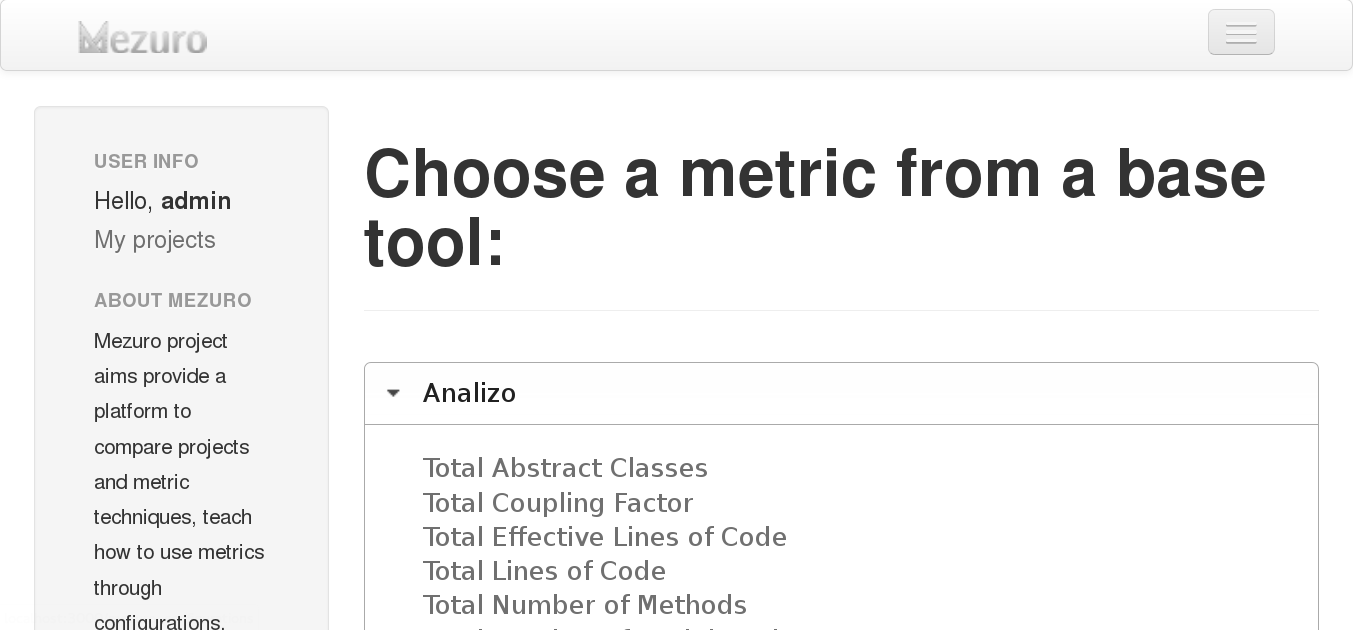
\includegraphics[width=\textwidth]{images/choose-metric.png}}
      \caption{Interface para escolha de ferramenta extratora de métrica e escolha desta para adicionar a uma configuração.}
      \label{fig:choose-metric}
    \end{figure}

    Criar uma configuração envolve 5 telas do sistema em 3 passos básicos:
    \begin{enumerate}
      \item Acessar a página de listagem de configurações;
      \item Clicando em ``New configuration'', preencher o formulário de criação de configuração e salvá-lo;
      \item Clicando em ``Add metric'', escolher a ferramenta de extração e qual a métrica a ser usada;
      \item Preencher o formulário (detalhado a seguir) e salvá-lo.
    \end{enumerate}

    Os passos 3 e 4 devem ser repetidos para cada métrica que deva ser adicionada à configuração. O formulário de métrica (passo 4) é complexo se comparado com o de configuração, mas, assim como os demais, cada campo possui detalhes sobre sua utilização. Aqui, destacamos os dois que consideramos os menos óbvios para um novo usuário:
    \begin{itemize}
      \item \textbf{Aggregation form:} Por exemplo, dada uma pasta com diversos arquivos contidos, como será calculada a nota desta pasta (média, mediana, máximo, mínimo, entre outras formas disponíveis);
      \item \textbf{ReadingGroup:} Conjunto de intervalos usado na interpretação da nota dada que dá um significado prático à nota calculada.
    \end{itemize}

    \subsubsection{Avaliação de repositório}

\section{Conclusão}

\newpage
\bibliographystyle{sbc}
\bibliography{mezuro}

\end{document}
